Bei den 140~\$ für das Zimmer hat es nicht mehr für ein Früh\-stück gereicht und so deckten wir uns im ört\-lichen Supermarkt ein.
Dazu gehörte das allerwichtigste über\-haupt, was man in diesem Land überhaupt braucht.
Keine Wumme, sondern Lippenbalsam!
Das gechlorte Leitungswasser setzt den Lippen und der Haut derart zu, dass man meinen könnte Nivea \& Co sponsoren das Chlor.

Danach ging es direkt auf den asphaltierten Wanderweg am Canyon.
Das ist er rund 2~km, denn viel weiter läuft der Durchschnittsamerikaner wahrscheinlich eh nicht.
Ab dann ist es ein typischer Wanderweg.
Wir sind vom Info-Zentrum bis fast zu \FOREIGN{Hermit's Rest} gelaufen, der einsetzende Regen und die deutlich längere Strecke ließ uns letztlich auf den Pendelbus aufspringen.

%links
%\newpage
\thispagestyle{empty}
\begin{tikzpicture}[remember picture, overlay]
\node[inner sep=0pt, yshift=.25\paperheight] at (current page.south) {%
	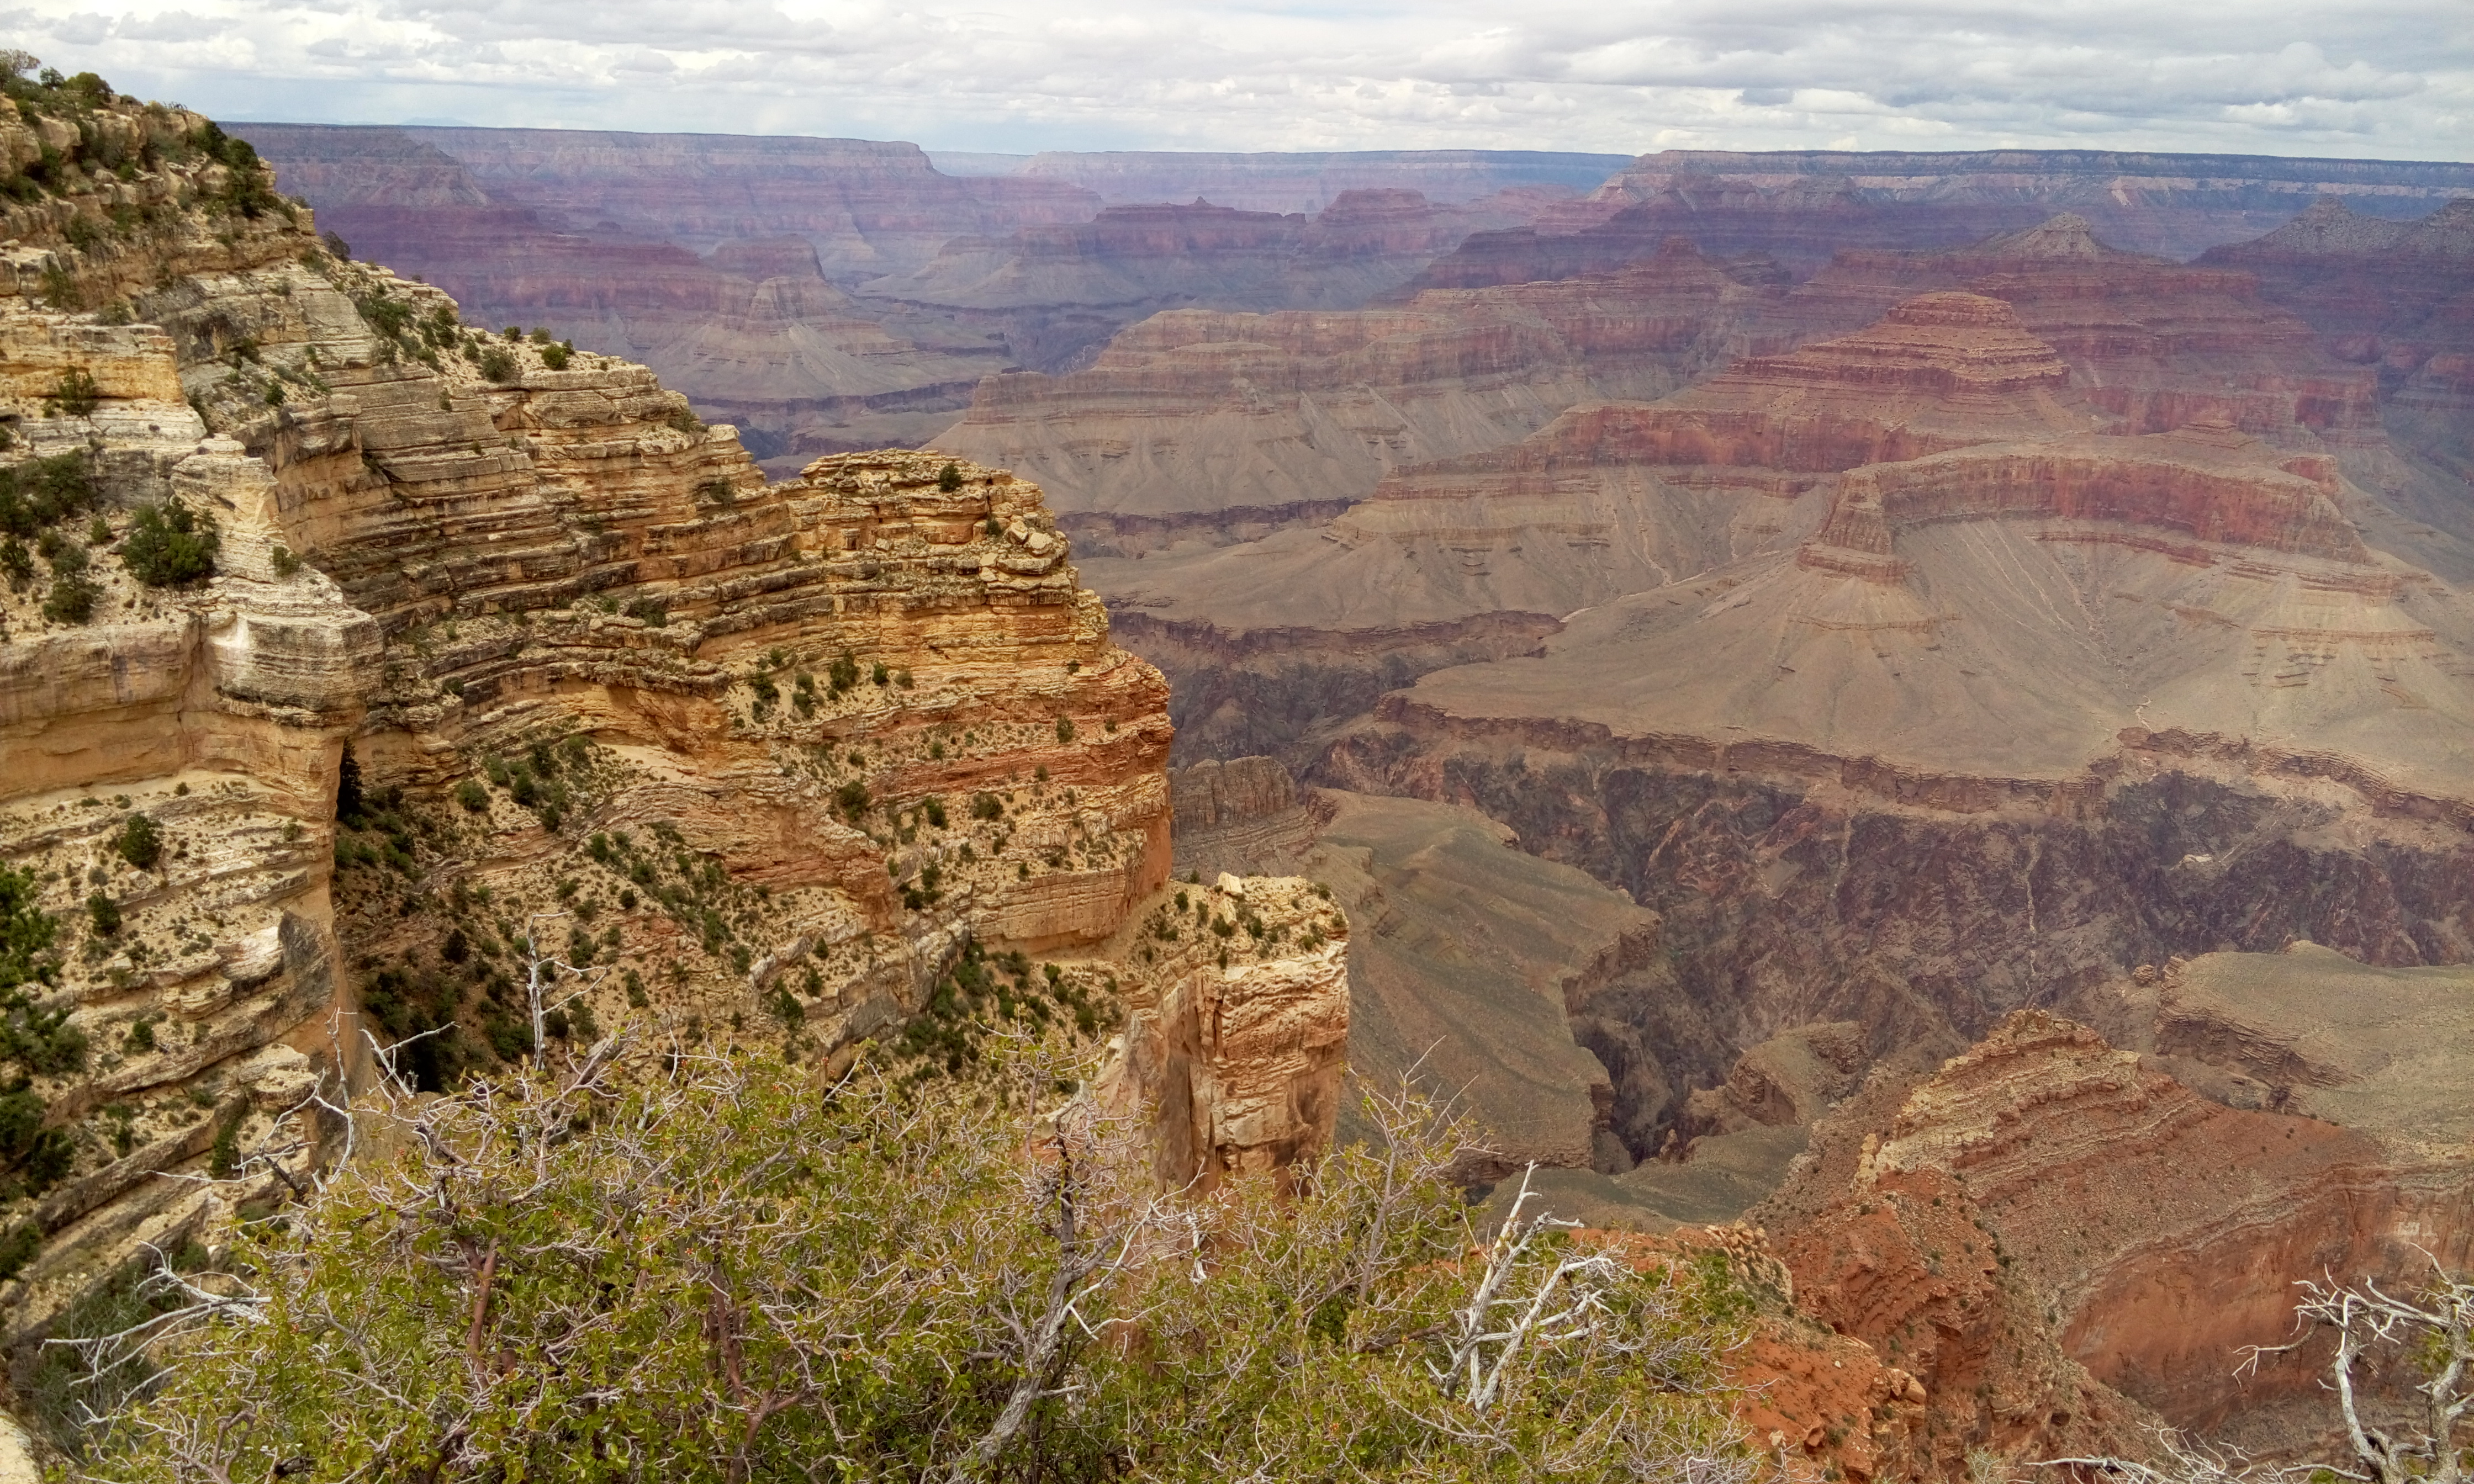
\includegraphics[width=\paperwidth,height=.5\paperheight]{10/image20160410_130723067.jpg};%
};
\end{tikzpicture}

%\vspace*{.4\paperheight}

\newpage

%rechts
%\thispagestyle{empty}
\begin{tikzpicture}[remember picture, overlay]
\node[inner sep=0pt, yshift=.25\paperheight] at (current page.south) {%
	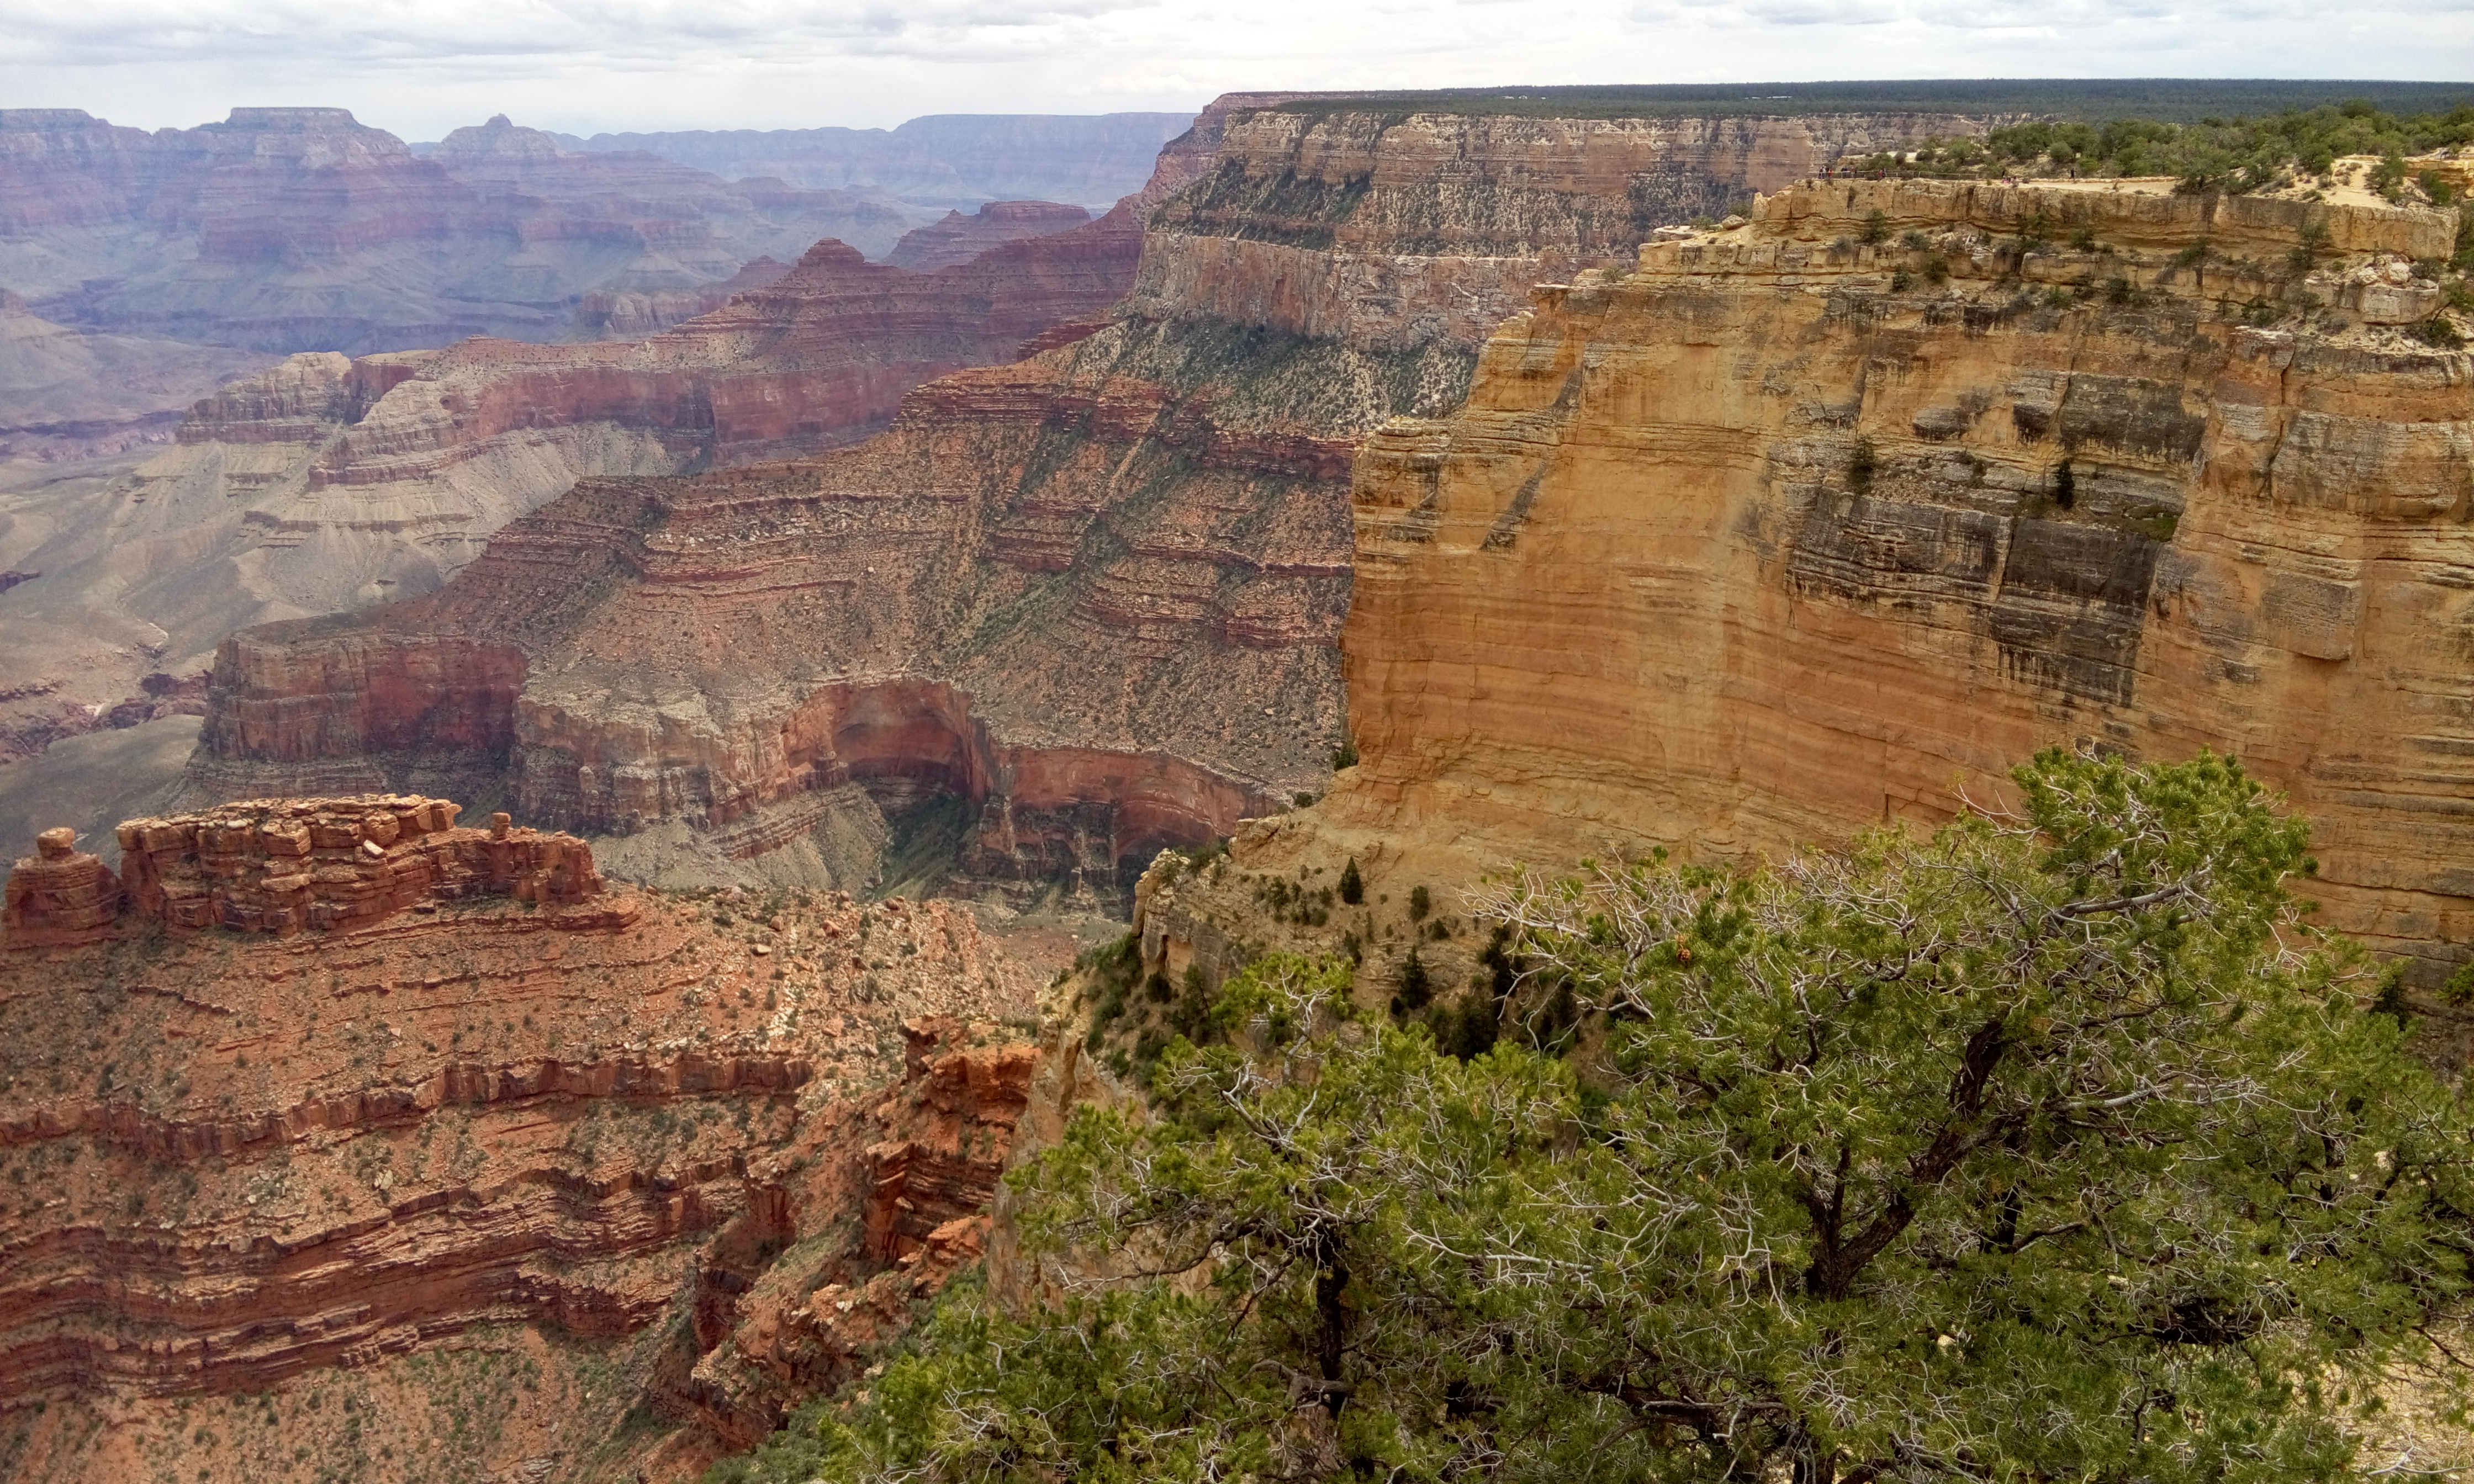
\includegraphics[width=\paperwidth,height=.5\paperheight]{10/image20160410_130709540.jpg};%
};
\end{tikzpicture}

%\vspace*{.4\paperheight}

Am \FOREIGN{South Rim} führen genau zwei Wege in den Canyon selbst.
Einer beim Besucherzentrum wofür nur ein paar Ureinwohner verjagt werden mussten und der andere ist das Lebenswerk des (kanadischen) Einsiedlers.
Im Canyon selbst liegt nochmal ein Hotel, wenn man die Wanderung vom \FOREIGN{South} zum \FOREIGN{North Rim} nicht in einem Zug machen möchte.
Allerdings muss man dafür mindestens neun Monate im Voraus reservieren.

%%\cleardoublepage{}
%\newpage
%\thispagestyle{empty}
%\begin{tikzpicture}[remember picture, overlay]
%\node[inner sep=0pt] at (current page.center) {%
%	\includegraphics[width=\paperwidth,height=\paperheight]{10/image20160410_120920455.jpg};%
%};
%%  \node[black,fill=white,text width=10em] (blub) at (0.5,0) {Distanz etwa 3.600~km}; %
%\end{tikzpicture}
%\newpage

Beeindruckt vom Grand Canyon ging es am Nachmittag weiter zum nächsten Staudamm, dem Hoover-Dam.
Wir kamen jedoch recht spät an und zu dieser Zeit war es untersagt den Damm zu Fuß zu betreten.
Der Hoover-Dam befindet sich zwischen den Bundesstaaten Arizona und Nevada was zur folge hat das man beim überqueren auch die Zeitzone wechselt.
So ging es die überschaubar vielen Meilen noch nach \TOWN{Las Vegas} weiter.

\newpage

Ich hatte ein paar Lichter in Form von Neonröhren erwartet, aber \FOREIGN{The Strip} ist mehr als nur ein paar Lichter.
Nachdem wir ins \FOREIGN{Treasure Island} eingecheckt hatten, sind wir am sehr späten Abend nochmal losgelaufen, um etwas zu essen.
Am \FOREIGN{Strip} finden sich in erster Reihe hauptsächlich Hotels, aber hier und da gibt es auch etwas Gastronomie.
Neben dem goldenden M fand sich ein mexikanischer, ein chinesischer und ein Pizza-Imbiss.
Selbstverständlich ist man offen für alles, doch dann fällt einem wieder ein, dass man im Heimatland stellenweise schon größte Probleme hat beim \glqq Ausländer\grqq \, etwas zu bestellen und dann auch noch das zu bekommen, was man wollte.
Folgerichtig gab es daher Pizza.
Calzone Meatball und Calzone Chesse.
Pizza zum Abgewöhnen.
